\section{Eliminazione delle generalizzazioni}
Di seguito viene mostrato come le generalizzazioni sono state eliminate per produrre
il {\it diagramma E-R ristrutturato}.

Nella totalità dei casi le generalizzazioni sono state eliminate {\bf accorpando
le entità figlie sull'entità padre}.

\vspace{15pt}

Nel caso della generalizzazione che coinvolge le entità {\tt Strumento}, {\tt Macchinario}
e {\tt Attrezzatura}, risulta comodo l'accorpamento sul padre in quanto {\tt Macchinario}
e {\tt Attrezzatura} non hanno attributi che il padre non possiede e non hanno
associazioni con altre entità.

\vspace{5pt}\centerline{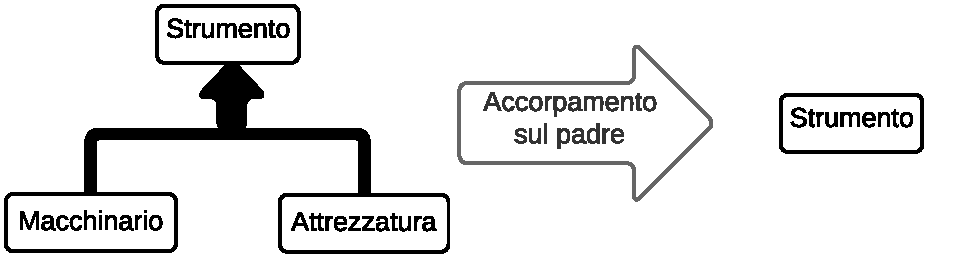
\includegraphics[width=\textwidth]{gen-strumento}}

\vspace{15pt}

Nel caso della generalizzazione che coinvolge le entità {\tt Menu} e  {\tt MenuPassato},
l'accorpamento sul padre porta soltanto all'aggiunta dell'attributo opzionale
{\tt DataFine}.

\vspace{5pt}\centerline{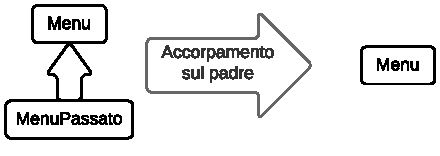
\includegraphics[width=0.8\textwidth]{gen-menu}}

\vspace{15pt}

Nel caso della generalizzazione che coinvolge le entità {\tt Comanda}, {\tt ComandaTavolo}
e {\tt ComandaTakeAway}, l'accorpamento sul padre non porta all'aggiunta di attributi opzionali.
Ma le associazioni {\tt Mittente} e {\tt Ordinazione} diventano opzionali ({\tt Richiesta} è
già opzionale). Non è necessario inserire qui un attributo {\tt Tipo} per riconoscere
il tipo di comanda in quanto può essere facilmente dedotto dalla presenza o meno
dell'associazione {\tt Ordinazione}.

\vspace{5pt}\centerline{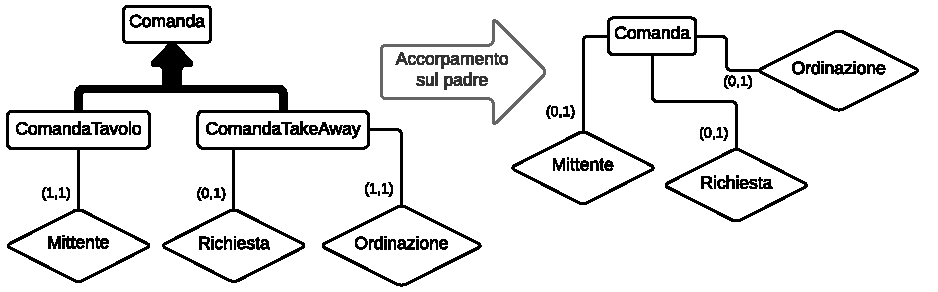
\includegraphics[width=\textwidth]{gen-comanda}}

\vspace{15pt}

Nel caso della generalizzazione che coinvolge le entità {\tt Gradimento}, {\tt GradimentoProposta}
e {\tt GradimentoSuggerimento}, l'accorpamento sul padre non porta all'aggiunta di attributi opzionali.
Ma le associazioni {\tt RiferimentoP} e {\tt RiferimentoS} diventano opzionali.
Non è necessario inserire qui un attributo {\tt Tipo} per riconoscere il tipo di
comanda in quanto può essere facilmente dedotto dall'associazione presente (se
{\tt RiferimentoP} o {\tt RiferimentoS}).

\vspace{5pt}\centerline{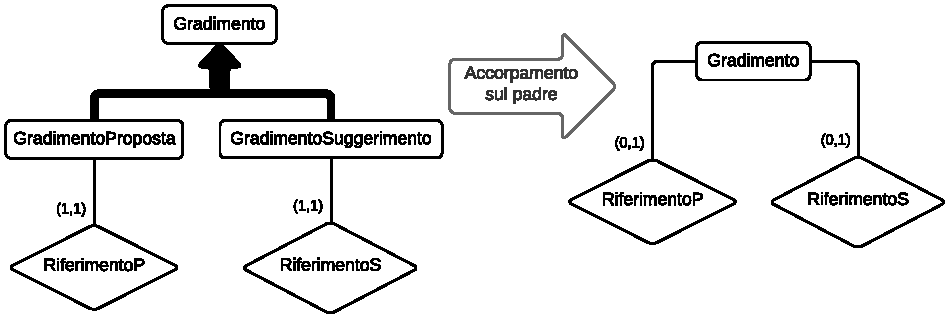
\includegraphics[width=\textwidth]{gen-gradimento}}

\vspace{15pt}

Nel caso delle due generalizzazioni che coinvolgono le entità {\tt Prenotazione},
{\tt PrenotazioneTelefonica}, {\tt PrenotazioneOnline} e {\tt Allestimento} si può
procedere con due accorpamenti sul padre: prima l'accorpamento di {\tt Allestimento}
su {\tt PrenotazioneOnline}; poi l'accorpamento di {\tt PrenotazioneTelefonica} e
{\tt PrenotazioneOnline} su {\tt Prenotazione}. Tutti gli attributi di {\tt PrenotazioneTelefonica}
e {\tt Allestimento} diventano opzionali, così anche le associazioni {\tt InvioPre}
e {\tt SerataTema}. % TODO: Si era deciso di usare un campo Tipo - ma perché? a me pare non serve

\vspace{5pt}\centerline{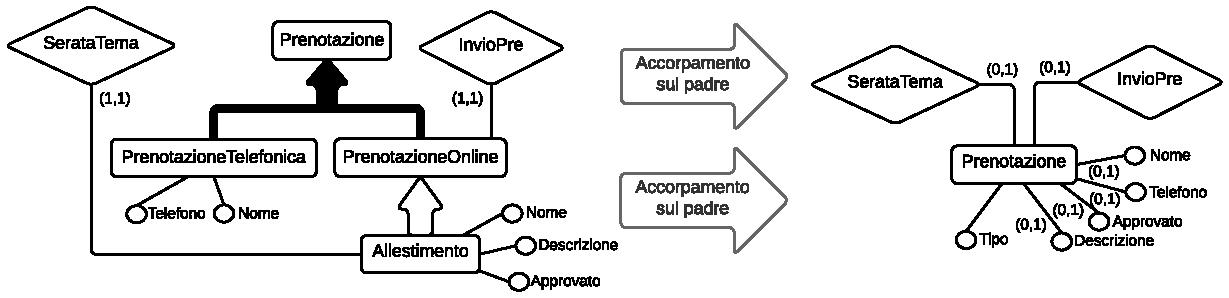
\includegraphics[width=\textwidth]{gen-prenotazione-allestimento}}
